% Options for packages loaded elsewhere
\PassOptionsToPackage{unicode}{hyperref}
\PassOptionsToPackage{hyphens}{url}
\PassOptionsToPackage{dvipsnames,svgnames,x11names}{xcolor}
%
\documentclass[
  10t,
]{article}

\usepackage{amsmath,amssymb}
\usepackage{iftex}
\ifPDFTeX
  \usepackage[T1]{fontenc}
  \usepackage[utf8]{inputenc}
  \usepackage{textcomp} % provide euro and other symbols
\else % if luatex or xetex
  \usepackage{unicode-math}
  \defaultfontfeatures{Scale=MatchLowercase}
  \defaultfontfeatures[\rmfamily]{Ligatures=TeX,Scale=1}
\fi
\usepackage{lmodern}
\ifPDFTeX\else  
    % xetex/luatex font selection
\fi
% Use upquote if available, for straight quotes in verbatim environments
\IfFileExists{upquote.sty}{\usepackage{upquote}}{}
\IfFileExists{microtype.sty}{% use microtype if available
  \usepackage[]{microtype}
  \UseMicrotypeSet[protrusion]{basicmath} % disable protrusion for tt fonts
}{}
\makeatletter
\@ifundefined{KOMAClassName}{% if non-KOMA class
  \IfFileExists{parskip.sty}{%
    \usepackage{parskip}
  }{% else
    \setlength{\parindent}{0pt}
    \setlength{\parskip}{6pt plus 2pt minus 1pt}}
}{% if KOMA class
  \KOMAoptions{parskip=half}}
\makeatother
\usepackage{xcolor}
\setlength{\emergencystretch}{3em} % prevent overfull lines
\setcounter{secnumdepth}{-\maxdimen} % remove section numbering
% Make \paragraph and \subparagraph free-standing
\makeatletter
\ifx\paragraph\undefined\else
  \let\oldparagraph\paragraph
  \renewcommand{\paragraph}{
    \@ifstar
      \xxxParagraphStar
      \xxxParagraphNoStar
  }
  \newcommand{\xxxParagraphStar}[1]{\oldparagraph*{#1}\mbox{}}
  \newcommand{\xxxParagraphNoStar}[1]{\oldparagraph{#1}\mbox{}}
\fi
\ifx\subparagraph\undefined\else
  \let\oldsubparagraph\subparagraph
  \renewcommand{\subparagraph}{
    \@ifstar
      \xxxSubParagraphStar
      \xxxSubParagraphNoStar
  }
  \newcommand{\xxxSubParagraphStar}[1]{\oldsubparagraph*{#1}\mbox{}}
  \newcommand{\xxxSubParagraphNoStar}[1]{\oldsubparagraph{#1}\mbox{}}
\fi
\makeatother


\providecommand{\tightlist}{%
  \setlength{\itemsep}{0pt}\setlength{\parskip}{0pt}}\usepackage{longtable,booktabs,array}
\usepackage{calc} % for calculating minipage widths
% Correct order of tables after \paragraph or \subparagraph
\usepackage{etoolbox}
\makeatletter
\patchcmd\longtable{\par}{\if@noskipsec\mbox{}\fi\par}{}{}
\makeatother
% Allow footnotes in longtable head/foot
\IfFileExists{footnotehyper.sty}{\usepackage{footnotehyper}}{\usepackage{footnote}}
\makesavenoteenv{longtable}
\usepackage{graphicx}
\makeatletter
\newsavebox\pandoc@box
\newcommand*\pandocbounded[1]{% scales image to fit in text height/width
  \sbox\pandoc@box{#1}%
  \Gscale@div\@tempa{\textheight}{\dimexpr\ht\pandoc@box+\dp\pandoc@box\relax}%
  \Gscale@div\@tempb{\linewidth}{\wd\pandoc@box}%
  \ifdim\@tempb\p@<\@tempa\p@\let\@tempa\@tempb\fi% select the smaller of both
  \ifdim\@tempa\p@<\p@\scalebox{\@tempa}{\usebox\pandoc@box}%
  \else\usebox{\pandoc@box}%
  \fi%
}
% Set default figure placement to htbp
\def\fps@figure{htbp}
\makeatother

% preamble.tex

% --- Document Structure and Layout ---

\usepackage[a4paper, total={6in, 8in}]{geometry}

% --- Paragraph settings ---

\setlength{\parindent}{0pt}
\setlength{\parskip}{6pt}

% --- Color Definitions ---

\usepackage[x11names]{xcolor} % Required for specifying custom colors, load before tcolorbox
\definecolor{headingblue}{RGB}{23,48,191}
\definecolor{boxtitle}{HTML}{F0F4F8}
\definecolor{boxbody}{HTML}{FBFDFF}
\definecolor{mainboxframe}{HTML}{F0F4F8}
\definecolor{subboxframe}{HTML}{F0F4F8}
\definecolor{crimson}{HTML}{880000}
\definecolor{monocolor}{RGB}{64,224,208}

% --- Fonts and Encoding ---

\usepackage{fontspec}         % Allows font specification
% \usepackage{amsmath}          % For math symbols

% Main Font
\setmainfont[
  UprightFont = *-Regular,
  ItalicFont = *-Italic,
  ItalicFeatures = { SmallCapsFont = *-Italic },
  SlantedFont = *-Regular,
  SlantedFeatures= { FakeSlant=0.2 },
  BoldFont = *-Bold,
  BoldFeatures = { SmallCapsFont = *-Bold },
  BoldItalicFont = *-BoldItalic,
  BoldItalicFeatures = { SmallCapsFont = *-BoldItalic },
  BoldSlantedFont= *-Bold,
  BoldSlantedFeatures= { FakeSlant=0.2, SmallCapsFont = *-Bold },
  SmallCapsFont = *-Regular,
  SmallCapsFeatures={ RawFeature=+smcp },
  Ligatures=TeX,
  Numbers={OldStyle, Proportional}
]{StixTwoText}

% Math Font
\setmathfont{StixTwoMath.otf}

% Monospace Font
\setmonofont[
  Scale=0.84
]{FiraCode Nerd Font}
\renewcommand{\ttfamily}{\small\fontspec{FiraCode Nerd Font}\color{DeepSkyBlue4}}
\renewcommand{\texttt}[1]{{\ttfamily #1}}

% --- Packages for Tables ---

\usepackage{array}            % For table column width specification
\usepackage{booktabs}         % For table rules
\usepackage{ragged2e}         % For text alignment (used with \newcolumntype)

% --- Headers and Footers ---

\usepackage{fancyhdr}
\pagestyle{fancy}
\renewcommand{\sectionmark}[1]{\markright{#1}{}}
\fancyhf{}
\fancyhead[LE,RO]{\thepage}
\fancyhead[LO]{\textsc{\MakeLowercase{\leftmark}}}
\fancyhead[RE]{\textsc{\MakeLowercase{\rightmark}}}

% --- Other Packages ---

\usepackage[version=4]{mhchem}% Formula subscripts using \ce{}

% --- Key Terms

\newcommand{\keyterm}[1]{\textsc{#1}}

%% Create a command for color emphasis
\newcommand{\highlight}[1]{\textcolor{crimson}{#1}}

% --- Boxes ---

% Define the mdframed environment
\usepackage{float}
\usepackage{mdframed}

% 1) Define a new float environment called "boxfloat"
\newfloat{boxfloat}{htbp}{lob}
\floatname{boxfloat}{Box}

% 3) Define the environment that wraps mdframed in a float
\newenvironment{boxedfloat}[2][]{%
  % Advance the box counter to produce "Chapter.BoxNo"
  \refstepcounter{boxcounter}%
  % Begin the float environment
  \begin{boxfloat}[htbp]
  % Begin the mdframed styling
  \begin{mdframed}[
    backgroundcolor=gray!5,
    innertopmargin=6pt,
    innerbottommargin=6pt,
    innerrightmargin=6pt,
    innerleftmargin=6pt,
    linewidth=0.25pt,
    linecolor=black,
    roundcorner=8pt,    % or 0pt if you prefer sharp corners
    skipabove=12pt,     % vertical space above the box
    skipbelow=12pt,     % vertical space below the box
    innermargin=0pt,
    outermargin=0pt
  ]%
    % Typeset the box heading: "Box 1.1. My Title"
    \setlength{\parindent}{0em}%
    \setlength{\parskip}{3pt}%
    \RaggedRight
    % Both "Box" and the user-supplied title are in small caps
    \small% switch the box contents to smaller text
    {\scshape Box \theboxcounter. #2}\par
    \vspace{6pt} % a little space after the heading
}{%
    \end{mdframed}
    \end{boxfloat}
}

% --- sansblock Environment ---

\usepackage{sourcesanspro}    % Load Source Sans Pro
\setsansfont{Source Sans Pro} % Set it as the sans-serif font
\newenvironment{sansblock}[1]
    {\small\sffamily\raggedright{\scshape #1}\ } % Ensure small caps for the title
  {} % End environment: no special commands needed

% --- Custom Column Type (using ragged2e) ---

\newcolumntype{R}[1]{>{\RaggedRight}p{#1}}

% ---  Margin Notes ---

\usepackage{marginnote}
\renewcommand*{\marginfont}{\footnotesize\itshape} % Style for margin notes

%% Set margin note outer margin to 0.7in
\setlength{\marginparwidth}{1.25in}

% --- Epigraph ---

\usepackage{epigraph}
\setlength\epigraphwidth{.9\textwidth}
\newenvironment{quotepara}
  {\itshape\raggedright\small\setlength{\parskip}{0.5em}} % Add small space between paragraphs
  {}
\renewcommand{\textflush}{quotepara}

%% Define a new epigraph environment without the horizontal rule and source/author
\newenvironment{simpleepigraph}
  {\begin{list}{}%
      {\setlength{\leftmargin}{2em}% Left margin
       \setlength{\rightmargin}{2em}% Right margin
       \setlength{\topsep}{1em}% Space above the epigraph
       \setlength{\itemsep}{0pt}% Space between items (irrelevant here)
       \setlength{\parsep}{0pt}}% Space between paragraphs
   \item\relax\raggedright\small} % Apply ragged-right and italic style for the epigraph text
  {\end{list}}

% --- Small Caps ---

\newcommand{\flatcaps}[1]{\textsc{\MakeLowercase{#1}}}

% --- Lists ---

%% General settings for all lists
\usepackage{enumitem}

% Global settings following Bringhurst's principles
% A global default to keep lists tight, but still allow subtle spacing:
\setlist{
  nosep,         % No extra space between items
  topsep=0.6em,  % A bit of space before/after the list
  parsep=0pt,
  partopsep=0pt
}

% First-level itemize (unordered) lists:
\setlist[itemize,1]{
  label=\textbullet,
  labelsep=0.4em,        % Space from bullet to text
  labelwidth=1em,        % Horizontal space set aside for bullet
  leftmargin=\dimexpr 1em + 0.4em\relax,
  itemindent=0pt,
  listparindent=0pt,
  align=left
}

% Second-level itemize, with a subtler symbol:
\setlist[itemize,2]{
  label=--,
  labelsep=0.4em,
  labelwidth=1em,
  leftmargin=\dimexpr 1em + 0.4em\relax,
  itemindent=0pt,
  listparindent=0pt,
  align=left
}

% First-level enumerate (ordered) lists:
\setlist[enumerate,1]{
  label=\arabic*.,
  labelsep=0.4em,
  labelwidth=1em,
  leftmargin=\dimexpr 1em + 0.4em\relax,
  itemindent=0pt,
  listparindent=0pt,
  align=left
}

% Second-level enumerate (letters, or you could do roman numerals):
\setlist[enumerate,2]{
  label=\alph*.,
  labelsep=0.4em,
  labelwidth=1em,
  leftmargin=\dimexpr 1em + 0.4em\relax,
  itemindent=0pt,
  listparindent=0pt,
  align=left
}

% --- Custom Chapter/Section Styles ---

\usepackage[compact]{titlesec} % Allows creating custom chapter styles
\titleformat{\chapter}[display]
  {\fontsize{60}{62}\bfseries}
  {\thechapter}
  {0pt}
  {\huge\noindent}
\titlespacing*{\chapter}{0pt}{0pt}{40pt}

\titleformat{\section}
  {\normalsize\normalfont}
  {\thesection}
  {0.6em}
  {\flatcaps}
\titlespacing*{\section}{0pt}{1\baselineskip}{1\baselineskip}

\titleformat{\subsection}[block]
  {\normalsize\normalfont} % defines the font size and style for the entire subsection heading, including both the number and the title
  {\thesubsection} % defines the format of the subsection number
  {1em} % the horizontal space between the subsection number and the title
  {\itshape} % defines the format of the subsection title itself
\titlespacing*{\subsection}{0pt}{1\baselineskip}{1\baselineskip}

\titleformat{\subsubsection}[runin]
  {\normalsize\normalfont} % defines the font size and style for the entire subsection heading, including both the number and the title
  {\thesubsubsection} % defines the format of the subsection number
  {1em} % the horizontal space between the subsection number and the title
  {\itshape}[.] % defines the format of the subsection title itself
\titlespacing*{\subsubsection}{0pt}{1\baselineskip}{1\baselineskip}

\titleformat{\paragraph}[runin]
  {\flatcaps}
  {\theparagraph}
  {0pt}
  {}

% --- Footnotes ---

\usepackage[norule,ragged,hang]{footmisc}  % Load footmisc with ragged option
\renewcommand{\footnotelayout}{\RaggedRight\footnotesize} % Typeset footnotes in \RaggedRight
\setlength{\footnotemargin}{1.5em}    % Adjust space between number and text
\makeatletter
\renewcommand{\@makefntext}[1]{%
    \parindent 1em%                    Set parindent for footnote text
    \noindent
    \hb@xt@ 1.8em{%                   Set hanging indent for footnote text
        \hss\@thefnmark.%
    }
    \RaggedRight #1%                 Typeset footnote text ragged right
}
\makeatother

% --- Captions ---

\usepackage{caption}
\captionsetup{
  font={small},
  labelfont={bf},
  textfont={},
  width=0.9\textwidth,
  justification=justified,
  labelformat=default,
  labelsep=period,
  format=plain
}
\renewcommand{\captionlabelfont}{\bfseries\scshape}

% --- Hyperlinks ---

\usepackage{hyperref}           % Load after most other packages, but before cleveref
\hypersetup{
    colorlinks=true,
    linkcolor=blue,
    filecolor=magenta,
    urlcolor=cyan,
    pdftitle={Overleaf Example},
    pdfpagemode=FullScreen,
    }

\urlstyle{same}

% --- Miscellaneous ---

%% Define a new command to print the current page number to the console
\ifluatex
  \usepackage{luacode}
  \usepackage{shellesc}
  \newcommand{\printpagenumber}{%
    \directlua{
      local pagenumber = tex.count.page
      print(string.format("Currently processing page: %d", pagenumber))
    }
  }
\fi

\usepackage{etoolbox}          % General package for patching commands
\usepackage{iftex}             % Detects the engine used
\usepackage{ellipsis}          % Fixes spacing around ellipses
\AddToHook{env/Highlighting/begin}{\small} % Set the code chunk font size globally

%% Use lining fonts
\newcommand\lining{\addfontfeatures{Numbers={Monospaced, Lining}}}
\AtBeginEnvironment{tabular}{\lining} % In tables
\renewcommand{\theequation}{ {\lining\arabic{equation}}} % For equation numbers

% --- Index (if needed) ---

\usepackage{makeidx}
\makeindex

% --- Other Typography Settings ---

\frenchspacing                % Single space after periods
\tolerance=400                % Default is 200; higher values allow more relaxed line-breaking.
\emergencystretch=3em         % Adds additional space to help line-breaking.
\hyphenpenalty=20             % Default is 50; lower values encourage hyphenation.

% --- Microtype Settings (adjust only if needed) ---

\usepackage{microtype}        % Improves typography
\microtypesetup{
   tracking = true,
   protrusion=true,
   expansion=true,
   factor = 1100,
   stretch = 15,
   shrink = 15
}

\makeatletter
\@ifpackageloaded{tcolorbox}{}{\usepackage[skins,breakable]{tcolorbox}}
\@ifpackageloaded{fontawesome5}{}{\usepackage{fontawesome5}}
\definecolor{quarto-callout-color}{HTML}{909090}
\definecolor{quarto-callout-note-color}{HTML}{0758E5}
\definecolor{quarto-callout-important-color}{HTML}{CC1914}
\definecolor{quarto-callout-warning-color}{HTML}{EB9113}
\definecolor{quarto-callout-tip-color}{HTML}{00A047}
\definecolor{quarto-callout-caution-color}{HTML}{FC5300}
\definecolor{quarto-callout-color-frame}{HTML}{acacac}
\definecolor{quarto-callout-note-color-frame}{HTML}{4582ec}
\definecolor{quarto-callout-important-color-frame}{HTML}{d9534f}
\definecolor{quarto-callout-warning-color-frame}{HTML}{f0ad4e}
\definecolor{quarto-callout-tip-color-frame}{HTML}{02b875}
\definecolor{quarto-callout-caution-color-frame}{HTML}{fd7e14}
\makeatother
\makeatletter
\@ifpackageloaded{caption}{}{\usepackage{caption}}
\AtBeginDocument{%
\ifdefined\contentsname
  \renewcommand*\contentsname{Table of contents}
\else
  \newcommand\contentsname{Table of contents}
\fi
\ifdefined\listfigurename
  \renewcommand*\listfigurename{List of Figures}
\else
  \newcommand\listfigurename{List of Figures}
\fi
\ifdefined\listtablename
  \renewcommand*\listtablename{List of Tables}
\else
  \newcommand\listtablename{List of Tables}
\fi
\ifdefined\figurename
  \renewcommand*\figurename{Figure}
\else
  \newcommand\figurename{Figure}
\fi
\ifdefined\tablename
  \renewcommand*\tablename{Table}
\else
  \newcommand\tablename{Table}
\fi
}
\@ifpackageloaded{float}{}{\usepackage{float}}
\floatstyle{ruled}
\@ifundefined{c@chapter}{\newfloat{codelisting}{h}{lop}}{\newfloat{codelisting}{h}{lop}[chapter]}
\floatname{codelisting}{Listing}
\newcommand*\listoflistings{\listof{codelisting}{List of Listings}}
\makeatother
\makeatletter
\makeatother
\makeatletter
\@ifpackageloaded{caption}{}{\usepackage{caption}}
\@ifpackageloaded{subcaption}{}{\usepackage{subcaption}}
\makeatother

\usepackage{bookmark}

\IfFileExists{xurl.sty}{\usepackage{xurl}}{} % add URL line breaks if available
\urlstyle{same} % disable monospaced font for URLs
\hypersetup{
  pdftitle={Artificial Intelligence for Academic Integrity (AI4AI)},
  pdfauthor={AJ Smit},
  colorlinks=true,
  linkcolor={blue},
  filecolor={blue},
  citecolor={blue},
  urlcolor={blue},
  pdfcreator={LaTeX via pandoc}}


\title{Artificial Intelligence for Academic Integrity (AI4AI)}
\author{AJ Smit}
\date{2025-03-17}

\begin{document}
\maketitle


\section{AI for Academic Integrity}\label{ai-for-academic-integrity}

AI supports academic work in various ways. Of specific interest are the
Generative Pre-trained Transformer (GPT) models, which can be used to
generate text, code, and other outputs. It can also operate on data,
images, and other forms of information. In this workshop, I will explore
some of the ways in which the GPT models can be used in our academic
research whilst keeping an eye on academic integrity.

\section{GPT Models}\label{gpt-models}

A variety of GPT models are available for use in academia. These models
include:

\begin{itemize}
\tightlist
\item
  \href{https://openai.com/}{\textbf{OpenAI}}

  \begin{itemize}
  \tightlist
  \item
    \textbf{GPT-4o-mini}\footnote{``o'' models are referred to as
      ``reasoning models''.}
  \item
    GPT-o1
  \item
    GPT-o1-mini
  \item
    GPT-o1-mini-high
  \item
    \textbf{GPT-o3-mini}
  \item
    \textbf{GPT-4o}
  \item
    GPT 4.5
  \item
    Has ``Customise ChatGPT'' option
  \end{itemize}
\item
  \href{https://www.anthropic.com/}{\textbf{Anthropic}}

  \begin{itemize}
  \tightlist
  \item
    \textbf{Claude 3.7 Sonnet}
  \item
    \textbf{Claude 3.5 Haiku}
  \item
    Two thinking modes: \textbf{Normal} and Extended
  \item
    Has ``Projects'' and ``Styles'' for customisation
  \end{itemize}
\item
  \href{https://one.google.com/intl/en_za/about/ai-premium/}{\textbf{Google
  Gemini}}

  \begin{itemize}
  \tightlist
  \item
    \textbf{Google Scholar}
  \item
    \textbf{2.0 Flash}
  \item
    \textbf{2.0 Flash Thinking}
  \item
    Gemini Advanced
  \item
    Deep Research
  \item
    Experimental models
  \item
    2.0 Pro
  \item
    \textbf{\href{https://notebooklm.google.com/}{NotebookLM}} (built on
    Gemini)
  \item
    NotebookLM Plus
  \item
    Option to use ``Gems''
  \end{itemize}
\item
  \href{https://scholarai.io/}{Scholar.AI}
\item
  \href{https://deepseek.ai/}{DeepSeek}
\item
  \href{https://www.perplexity.ai/}{Perplexity}
\item
  \href{https://consensus.app/}{Consensus}
\item
  \href{https://www.thesisai.io/}{Thesis.AI}
\item
  \textbf{\href{https://github.com/features/copilot}{GitHub Copilot}},
  available to all academic users with a GitHub account. It is
  accessible via the RStudio interface.
\end{itemize}

These models have their distinct ``personalities'', but they also have
various personalisation options to help ``humanise'' their writing. In
this workshop, we will go over the strengths and weaknesses of all these
models, and we will look at how to customise them in ways that will
improve academic integrity and bring them in line with how people
\emph{actually} write.

Many new AI models appear each day, some with the needs of academics in
mind. For example, \href{https://elicit.com/}{Elicit},
\href{https://www.researchrabbit.ai/}{ResearchRabbit}, and
\href{https://www.scholarcy.com/}{Scholarcy} also support the type and
style of writing we do. Many also help us make sense of a bewildering
body of peer-reviewed research papers. I'll spend less time with these,
but the basic principles that apply to the GPTs developed for general
consumption work here too.

\section{The Importance of Prompts}\label{the-importance-of-prompts}

Prompts are important in guiding the AI to generate the desired output.
The better the prompt, the better the output. Asking insightful,
well-informed, detailed, and descriptive questions will lead to better
results. Aksing questions as a 10-year old would will lead to poor
results. In AI, there really is such a thing as a dumb question! In this
part of the workshop, I will discuss the importance of prompts and how
to ask good questions.

\subsection{Setting up your writing style and prior
expectations}\label{setting-up-your-writing-style-and-prior-expectations}

An example pre-configuration of the AI for your writing style and prior
expectations is as follows:

\begin{tcolorbox}[enhanced jigsaw, colback=white, rightrule=.15mm, opacityback=0, left=2mm, leftrule=.75mm, colframe=quarto-callout-note-color-frame, arc=.35mm, bottomrule=.15mm, breakable, toprule=.15mm]
\begin{minipage}[t]{5.5mm}
\textcolor{quarto-callout-note-color}{\faInfo}
\end{minipage}%
\begin{minipage}[t]{\textwidth - 5.5mm}

\vspace{-3mm}\textbf{ChatGPT profile}\vspace{3mm}

Think step-by-step, showing reasoning for complex problems.

Break down complex tasks and ask clarifying questions, if needed. Ask me
if you are unclear.

Aim to be scholarly, confident, and analytical, appealing to readers
accustomed to advanced academic dialogue. Maintain a poised authority,
weaving scientific depth without slipping into empty verbosity. While
the vocabulary reflects complexity -- e.g.~``epistemic,'' ``conceptual
ordering,'' ``structured inference,'' and ``rigorous standard'' -- do
not use jargon for its own sake. Emphasise clarity that respects the
reader's intelligence and allows concepts to resonate without
condescension.

Let the sentence structure shift between long, layered forms that
contextualise, define, and critically engage, and shorter, sharper
sentences that reinforce key arguments and points. Use a variety of
clauses, parenthetical asides, and em-dashes to give the writing a
dynamic flow. This rhythmic variation and precise diction shape a voice
that rewards a close, attentive reading.

Some phrases recur to define the analytical approach, e.g.,
``particularly,'' ``structured inference,'' ``conceptual groundwork,''
``rigorous standard,'' ``systematic reasoning,'' ``intellectual
milieu,'' and ``distinguish signal from noise.'' Constructions like
``laid the foundation for,'' ``conceptual leap,'' and ``philosophical
tradition'' emphasise historical continuity and highlight how earlier
ideas inform contemporary discourse.

Avoid these words: particularly, crucial(ly), essential, holistic,
especially, challenge(s), sophisticated, ensuring/ensure, profound,
remarkable, nuanced, emerge(s), questioning, nudge(s), robust, ``stand
out,'' ``by acknowledging,'' ``It's a reminder,'' ``In summary.''

Aim for a
\href{https://en.wikipedia.org/wiki/Gunning_fog_index}{Gunning-Fog
index} above 23, and use British English.

Avoid words that flatten complexity or imply hollow emphasis. Rely on
carefully chosen terms that reflect a style suited to readers ready to
engage with advanced scholarly thought.

Avoid excessive political correctness, overly polite answers, being
apologetic, or always assuming I am correct. I appreciate being argued
or disagreed with.

I like a detailed, critical analysis. I dislike bullet points (unless
absolutely necessary). I value long-form writing. I dislike formulaic
responses, like paragraphs of equal length --- keep them varied. Avoid
the concluding paragraph starting with ``In summary\ldots{}''. In fact,
avoid these silly summary paragraphs altogether.

\end{minipage}%
\end{tcolorbox}

\subsection{Write detailed prompts}\label{write-detailed-prompts}

\begin{tcolorbox}[enhanced jigsaw, colback=white, rightrule=.15mm, opacityback=0, left=2mm, leftrule=.75mm, colframe=quarto-callout-note-color-frame, arc=.35mm, bottomrule=.15mm, breakable, toprule=.15mm]
\begin{minipage}[t]{5.5mm}
\textcolor{quarto-callout-note-color}{\faInfo}
\end{minipage}%
\begin{minipage}[t]{\textwidth - 5.5mm}

Be as verbose and explicit as you can be when writing your prompts.
Provide all the necessary background information, and be specific about
what you want the AI to do. For example, instead of asking ``What is the
impact of climate change on marine ecosystems?'', you could ask ``Can
you provide a detailed analysis of how climate change affects marine
ecosystems, including changes in temperature, ocean acidification, and
shifts in species distribution? Please include recent research findings
and examples from different regions.'' This will give you a reasonable
chance of getting a more detailed and relevant response.

But to be even more effective, try constructing a prompt like this one:

\subsection{Example 1}\label{example-1}

A recent method adapted from the marine heatwave and marine cold spell
detection methodology integrates high-resolution SST data from multiple
products with wind measurements. The method works by detecting
simultaneous increases in south-easterly winds and corresponding
decreases in SST, which signal the occurrence of upwelling. By
calculating metrics like intensity (magnitude of SST drops), duration
(length of time the event persists), and frequency (how often upwelling
events occur), the authors create a comprehensive tool for evaluating
upwelling dynamics.

The metrics are calculated on the SST data, where an upwelling event
(henceforth `event') is signalled by the drop in SST below a threshold,
i.e.~``If the temperature dropped {[}below{]} the seasonally varying
25th percentile of SST for a particular site, we deemed this a
confirmation of the occurrence of an upwelling event at that site.'' So,
an event is detected as TRUE when this drop occurs and persists for a
day or more. I think that more frequent and longer-lasting events will
lower SST during the upwelling season. If, over time (decades),
upwelling events become more frequent and longer lasting, it will be
accompanied by a decadal shift (lowering) in SST.

The paper that developed this methodology studied these upwelling events
in conjunction with ``simultaneous increases in south-easterly winds.''
They did not use wind stress curl, which could be a significant
omission. Could wind stress curl better predict SST and upwelling event
metrics than simply looking at the incidence of south-easterly winds?

Please provide an analysis of the above synopsis of my proposed research
approach. Also, address these questions in the process:

\begin{enumerate}
\def\labelenumi{\arabic{enumi}.}
\tightlist
\item
  How can one use quantile regression to study this problem (i.e., wind
  stress curl as a driver of SST and upwelling event metrics)?
\item
  Is quantile regression the best approach to use?
\item
  How would one determine the threshold below which SST drops when
  signalled as an upwelling event?
\item
  Any other considerations?
\end{enumerate}

\end{minipage}%
\end{tcolorbox}

You could use a synthesis obtained through some deep literature review
as input for developing a structure for your thesis or paper. For
example, using AI output generated earlier, you could ask:

\begin{tcolorbox}[enhanced jigsaw, colback=white, rightrule=.15mm, opacityback=0, left=2mm, leftrule=.75mm, colframe=quarto-callout-note-color-frame, arc=.35mm, bottomrule=.15mm, breakable, toprule=.15mm]
\begin{minipage}[t]{5.5mm}
\textcolor{quarto-callout-note-color}{\faInfo}
\end{minipage}%
\begin{minipage}[t]{\textwidth - 5.5mm}

\vspace{-3mm}\textbf{Example 2}\vspace{3mm}

Please look at this breakdown of knowledge about kelp forests (pasted
below) and suggest only four or five main headings (excluding
subheadings) under which to discuss the status of knoweldge about kelp
globally:

\begin{itemize}
\tightlist
\item
  \textbf{Kelp Forest Ecology} Kelp forests are conspicuously dominated
  by large brown algae and reflect a high degree of biological
  organization. Kelp ecosystems have been the focus of much research
  because of the complexity of biological interactions that structure
  them. Kelp forests provide biogenic habitat that can enhance diversity
  and productivity both locally and over broader spatial scales through
  detrital subsidy.
\item
  \textbf{Kelp Species and Distribution} Kelp species of \emph{Ecklonia
  maxima} and \emph{Laminaria pallida} are commonly found along the west
  coast of southern Africa. \emph{E. maxima} and \emph{L. schinzii} are
  found between the mean low water level and 15 meters below on rocky
  exposed shores, while \emph{L. pallida} occupies areas of lower
  hydrodynamic stress. Molecular tools are being used to test hypotheses
  regarding kelp evolutionary biogeography, in part because kelps have
  sufficient dispersal barriers to enable the study of their evolution
  based on present-day distributions.
\item
  \textbf{Kelp Primary Production and Carbon Cycling} Kelp forests are
  among the most prolific primary producers on the planet, supporting
  productivity per unit area that rivals that of tropical rainforests.
  Kelp forests play a significant role in coastal carbon cycles. Rates
  of carbon assimilation in \emph{Ecklonia radiata} forests can rival
  those of giant kelp forests and \emph{Laminaria} forests.
\item
  \textbf{Kelp-Associated Communities} Numerous faunal species use the
  epiphytic algae associated with the stipe of \emph{Laminaria
  hyperborea} as habitat and a food source. Kelp beds in the southern
  Benguela are associated with about 30 species, many of which are
  fished commercially or recreationally.
\item
  \textbf{Kelp and Fisheries} Changes in kelp density and/or area
  influence the abundance and diversity of associated fisheries. Kelp
  presence and density have an actual effect on associated fisheries.
\item
  \textbf{Kelp Forest Monitoring} Macroalgae are utilized as biological
  indicators of ecosystem health in many monitoring programs worldwide.
  Macroalgae mapping can be carried out through direct observation or by
  indirect methods using remote sensing techniques.
\item
  \textbf{Threats to Kelp Ecosystems} Factors such as climate change,
  overfishing, and invasive species threaten kelp forest ecosystems.
  Darkening in coastal seas associated with increased turbidity results
  in both reduced biomass and depth distribution, and lower productivity
  of \emph{E. radiata}.
\end{itemize}

\textbf{Gaps in Knowledge and Future Research Directions:}

\begin{itemize}
\tightlist
\item
  \textbf{Fate of fixed carbon} A comprehensive understanding of the
  fate of fixed carbon in kelp forests is lacking. Future research
  should focus on the mechanisms of transport, decomposition,
  re-mineralization and burial of kelp-derived organic matter and how
  these may be impacted by anthropogenic- and climate- related changes
  in the environment.
\item
  \textbf{Kelp-fisheries interactions} There are methodological,
  geographical, and logistical gaps that should be filled in order to
  get a broader understanding of interactions between kelp beds and
  fisheries.
\item
  \textbf{South African Kelp Ecosystems} Since the Kelp Bed Ecology
  Programme of the 1970s and 1980s, there has been no concentrated
  research effort afforded to South African kelp ecosystems. Future
  research directions are likely to be centered around the impacts of
  climate change, overfishing and invasive species on kelp forest
  ecosystems.
\item
  \textbf{Harmonization of Marine Macroalgal Monitoring} There is a need
  to harmonize marine macroalgal monitoring, identifying common metrics
  and approaches in sampling design, field measurements, taxonomic
  resolution and data management, in order to develop standardized
  procedures which may allow data obtained to be compared.
\end{itemize}

\end{minipage}%
\end{tcolorbox}

Use AI to generate some synthetic data which you may use to develop,
test, and implement an unknown statistical method. Again, giving it a
full, detailed background to start its reasoning from will get you much
further:

\begin{tcolorbox}[enhanced jigsaw, colback=white, rightrule=.15mm, opacityback=0, left=2mm, leftrule=.75mm, colframe=quarto-callout-note-color-frame, arc=.35mm, bottomrule=.15mm, breakable, toprule=.15mm]
\begin{minipage}[t]{5.5mm}
\textcolor{quarto-callout-note-color}{\faInfo}
\end{minipage}%
\begin{minipage}[t]{\textwidth - 5.5mm}

\vspace{-3mm}\textbf{Example 3}\vspace{3mm}

\textbf{Your initial prompt:} We can measure algal nutrient uptake rates
using two types of experiments: multiple flask experiments and
perturbation experiments. The fundamental concept underlying both
methods is to introduce a known quantity of nutrients (termed the
substrate) into a flask or a series of flasks and then measure the rate
of nutrient uptake (\(V\)) at different substrate concentrations
(\([S]\)). We calculate the nutrient uptake rate as the change in
nutrient concentration in the flask over a predefined time interval
(\(V = \Delta [S]/\Delta t\)). Consequently, both experiments generate
data that relate the nutrient uptake rate to the corresponding substrate
concentration. The primary difference between the two methods lies in
the experimental setup and the data analysis.

In the \textbf{multiple flask method}, we prepare a series of flasks,
each containing a different initial concentration of the substrate
nutrient to span the range typically encountered by the specimen in its
natural environment. We then measure the nutrient uptake rate in
\emph{each individual flask} over a specific time period, for example by
taking measurements at the start (\(t=0\)) and end (\(t=30\) minutes) of
the incubation. We calculate the change in substrate concentration over
this time interval in each flask to determine the corresponding nutrient
uptake rate. The resulting data from this method therefore consists of
the different initial substrate concentrations used in each flask,
paired with their respective measured nutrient uptake rates over the
incubation period.

What statistical test yould you recommend?

\textbf{The next iteration on the first prompt} Let's go with the
Michaelis-Menten model.

I use R. Use a simulated dataset and demonstrate how to fit the MM model
to the hypothetical uptake data.

\textbf{And then refine it further} Below I will paste the output of the
non-linear regresssion you suggested (as above). Please write up these
findings in English suitable for the results section in a publications
(e.g.~the journal Marine Biology):

\texttt{Formula:\ V\ \textasciitilde{}\ (Vmax\ *\ S)/(Km\ +\ S)}

\texttt{Parameters:}
\texttt{Estimate\ Std.\ Error\ t\ value\ Pr(\textgreater{}\textbar{}t\textbar{})}

\texttt{Vmax\ \ \ 9.7239\ \ \ \ \ 0.3907\ \ 24.891\ 2.14e-15\ ***}

\texttt{Km\ \ \ \ \ 0.8621\ \ \ \ \ 0.1297\ \ \ 6.647\ 3.08e-06\ ***}

\texttt{-\/-\/-}

\texttt{Signif.\ codes:\ \ 0\ ‘***’\ 0.001\ ‘**’\ 0.01\ ‘*’\ 0.05\ ‘.’\ 0.1\ ‘\ ’\ 1}

\texttt{Residual\ standard\ error:\ 0.4873\ on\ 18\ degrees\ of\ freedom}

\texttt{Number\ of\ iterations\ to\ convergence:\ 4}
\texttt{Achieved\ convergence\ tolerance:\ 1.493e-07}

\end{minipage}%
\end{tcolorbox}

Use AI to develop a specific data analysis worflow suitable to your
task. Point to specific localities on your computer where the data
reside, and be as informative as possible about the nature of the data,
including what the variables are called, etc. Although the resulting R
script will not run on the AI system, it will be a good starting point
for you to adapt and run on your own computer (possibly involving
subsequent steps of iterating through AI). For example, you could ask:

\begin{tcolorbox}[enhanced jigsaw, colback=white, rightrule=.15mm, opacityback=0, left=2mm, leftrule=.75mm, colframe=quarto-callout-note-color-frame, arc=.35mm, bottomrule=.15mm, breakable, toprule=.15mm]
\begin{minipage}[t]{5.5mm}
\textcolor{quarto-callout-note-color}{\faInfo}
\end{minipage}%
\begin{minipage}[t]{\textwidth - 5.5mm}

\vspace{-3mm}\textbf{Example 4}\vspace{3mm}

I have created a grid template with a predefined spatial extent and
resolution as follows:

\texttt{template\_grid\ \textless{}-\ expand.grid(lon\ =\ seq(11,\ 20,\ by\ =\ lon\_increment),\ lat\ =\ seq(-35,\ -17,\ by\ =\ lat\_increment))}

I need to regrid MUR SST data, which are situated at
``/Volumes/OceanData/Tom/MUR'' as a series of .rds files.

The content of the .rds files is the variables ``lon'', ``lat'', ``t''
(time, in Date format, e.g.~``2014-06-02''), and ``temp'' (sea surface
temperature).

I want to regrid these files to the \texttt{template\_grid} and collect
all the data in one combined .Rdata file at the end.

Please provide an R script to accomplish this.

\end{minipage}%
\end{tcolorbox}

For lecturers, use it to make sense of student tasks and assignments
submitted on iKamva. For example, you could ask to extract marks for
self-assessed assignments from a set of files. Ask the AI to look for
specific keywords in the text, or to extract specific information from
the text. As an example:

\begin{tcolorbox}[enhanced jigsaw, colback=white, rightrule=.15mm, opacityback=0, left=2mm, leftrule=.75mm, colframe=quarto-callout-note-color-frame, arc=.35mm, bottomrule=.15mm, breakable, toprule=.15mm]
\begin{minipage}[t]{5.5mm}
\textcolor{quarto-callout-note-color}{\faInfo}
\end{minipage}%
\begin{minipage}[t]{\textwidth - 5.5mm}

\vspace{-3mm}\textbf{Example 5}\vspace{3mm}

Please create a Python script to accomplish the following:

The directory
`/Users/ajsmit/Library/CloudStorage/Dropbox/BCB744/2025/sandbox' has the
following subdirectories, e.g.:

`Task A' \textgreater{} `MCCOMB, JODY(3650596)' \textgreater{}
`Submission attachment(s)' \textgreater{}
`task\_a\_completed\_by\_jody\_mccomb\_3650596.R'

or

`Task A Self-Assessment' \textgreater{} `MCCOMB, JODY(3650596)'
\textgreater{} `Submission attachment(s)' \textgreater{}
`task\_a\_completed\_by\_jody\_mccomb\_3650596.xlsx'\,'

etc.

\begin{enumerate}
\def\labelenumi{\arabic{enumi}.}
\item
  Delete all files named `timestamp.txt'
\item
  Find all the files with extensions `.R', `.html', `.xlsx', `.qmd',
  `.pdf', `docx', or `.txt' in these subdirectories and rename them to
  e.g., 'MCCOMB, JODY(\_3\_6\_5\_0\_59\_\_6).R' or 'MCCOMB,
  JODY(\_3\_6\_5\_0\_59\_\_6).xlsx' (this is the student Surname, Name
  (Student\_no) and the file extension). Most of these details are
  supplied in the naming scheme of the subdirectories, as indicated in
  the examples.
\item
  Copy all these renamed files in `Task A' and `Task A Self-Assessment'
  to `Task A processed'. Similarly, renamed files in `Task B' and `Task
  B Self-Assessment' will be copied to `Task B processed', etc.
\item
  Remove all the original subdirectories, e.g.~`Task A' \textgreater{}
  'MCCOMB, JODY(\_3\_6\_5\_0\_59\_\_6)' \textgreater{} `Submission
  attachment(s)' and any remaining files within any level of these
  subdirectories.
\end{enumerate}

\end{minipage}%
\end{tcolorbox}

\begin{tcolorbox}[enhanced jigsaw, colback=white, rightrule=.15mm, opacityback=0, left=2mm, leftrule=.75mm, colframe=quarto-callout-note-color-frame, arc=.35mm, bottomrule=.15mm, breakable, toprule=.15mm]
\begin{minipage}[t]{5.5mm}
\textcolor{quarto-callout-note-color}{\faInfo}
\end{minipage}%
\begin{minipage}[t]{\textwidth - 5.5mm}

\vspace{-3mm}\textbf{Example 6}\vspace{3mm}

The attached image show a maximum covariance analysis on two gridded
fields: SST and eddy kinetic energy over the period 2013 to 2022. The
timeseries was detrended prior to analysis. Please help me understand
how to interpret this figure.

\textless Also paste the image you want AI to analyse\ldots,
e.g.\textgreater{}
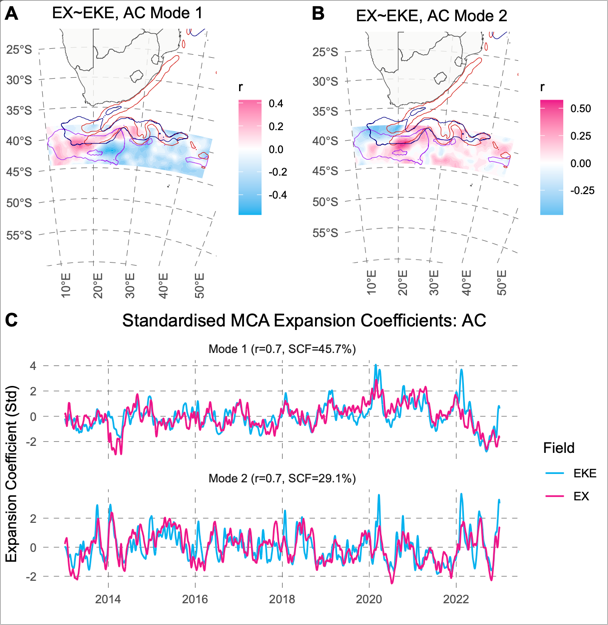
\includegraphics[width=0.8\linewidth,height=\textheight,keepaspectratio]{MCA.png}

\end{minipage}%
\end{tcolorbox}

\section{Applications of AI in Academic
Work}\label{applications-of-ai-in-academic-work}

Now that we understand the diversity of GPT models, their common basis
of operation, and the importance of prompts, I will look at some of the
ways in which we can use AI in our academic work. By way of examples,
I'll cover the following topics:

\subsection{Research and Working With
Ideas}\label{research-and-working-with-ideas}

\begin{itemize}
\tightlist
\item
  Literature reviews: Gemini Advanced and Perplexity's deep research;
  SciSpace Deep Review for focussing solely on academic sources and
  finding more relevant papers faster, and to export references

  \begin{itemize}
  \tightlist
  \item
    Finding relevant papers
  \item
    Summarising papers
  \item
    Extracting key points
  \item
    Generating literature reviews
  \item
    Writing literature reviews
  \end{itemize}
\item
  Structuring and mapping our ideas and thoughts

  \begin{itemize}
  \tightlist
  \item
    Outlining
  \item
    Mind mapping
  \item
    Concept mapping
  \item
    Structuring papers
  \end{itemize}
\item
  Brainstorming ideas
\item
  Deeper research
\item
  Facilitate interdisciplinary collaboration
\item
  Staying updated on research trends
\item
  Summarise influential researchers
\item
  Help with public outreach and science communication
\end{itemize}

\subsection{Writing}\label{writing}

\begin{itemize}
\tightlist
\item
  Rewriting
\item
  Summarising
\item
  Paraphrasing
\item
  Generating text
\item
  Validating ideas, concepts, and factual accuracy
\item
  Reviewing
\item
  Editing
\item
  Proofreading
\item
  Referencing (!)
\end{itemize}

\subsection{Data}\label{data}

\begin{itemize}
\tightlist
\item
  Cleaning
\item
  Extracting data from PDFs 9tables, figures, etc.)
\item
  Scripting (e.g., R, Python)

  \begin{itemize}
  \tightlist
  \item
    convert English to code
  \item
    convert code to English
  \item
    problem solving (statistics and data analysis)
  \item
    visualising
  \item
    debugging
  \end{itemize}
\item
  Interpreting and double-checking findings
\end{itemize}

\subsection{Personal Assistant}\label{personal-assistant}

\begin{itemize}
\tightlist
\item
  Writing applications (building on existing work, adapting, updating)
\item
  Writing emails (language, etc.)
\item
  Others
\end{itemize}

\section{Specific Workflows}\label{specific-workflows}

The general strategy across all three academic outputs emphasises the
proactive and intelligent use of AI tools to streamline research,
enhance the quality of the work, and ensure adherence to academic best
practices. Use these tools not just for basic information retrieval but
for deeper analysis, identification of gaps, methodological awareness,
and critical self-assessment.

\subsection{A Literature Review}\label{a-literature-review}

\begin{itemize}
\tightlist
\item
  Define the specific area (clear \textbf{topic} and/or \textbf{research
  questions}, increasing granularity to \textbf{aims} and
  \textbf{objectives}) or question that your literature review will
  address.
\item
  Use \textbf{deep research tools} to conduct a broad search of the
  knowledge base, and at this early stage you might not yet focus on the
  peer reviewed literature. This is where you can use the AI to help you
  develop a broad overview of the topic. You can also use it to
  \textbf{generate a list of keywords and phrases that are relevant to
  your topic}. This will help you refine your formal literature search
  terms and find more specific peer-reviewed papers.
\item
  Now, find the references. I prefer plain, old-fashioned \textbf{Google
  Scholar}, but you could use AI tools like \textbf{Gemini Advanced},
  \textbf{Perplexity}, or \textbf{SciSpace} Deep Review to conduct broad
  searches and gather relevant academic sources. Tools like SciSpace are
  specifically designed for academic sources as they return only
  peer-reviewed papers. They also allow you to export references to your
  reference manager. \textbf{Consensus} is a great tool for finding the
  consensus on a topic, and it can also help you find relevant papers.
  But keep the fallibility of these systems in mind.
\item
  \textbf{Find PDF copies} each and every reference that the above AI
  (and manual) searches reveal. Tools like Perplexity and Gemini link
  back to the original sources, but you need to verify them. SciSpace
  allows for easy export to reference managers. {\textbf{Check each fact
  yourself!}}
\item
  Use the AI to \textbf{generate summaries} of the existing literature
  to get a broad understanding of the field and identify key themes and
  arguments. Here, \textbf{NotebookLM} is your friend. Depending on the
  topic, you may instruct the AI to focus on specific aspects, such as
  methodology, findings, or theoretical frameworks. As always, being
  very specific in your prompts will yield better results -- it helps to
  already know the framework of the output that you are looking for.
  Discuss this with your supervisor or colleagues.
\item
  Based on the initial output, you may refine your search terms and use
  filters (e.g., publication date, methodology, journal quality) to
  narrow down the most relevant and high-quality studies. Consensus is
  useful for understanding the consensus and quality of research.
\item
  Look for \textbf{recurring themes}, \textbf{significant findings}, and
  \textbf{trends} in the literature. Develop an understanding of
  \textbf{how the field has changed and developed since its inception}.
  What are the \textbf{gaps}? What are the \textbf{opportunities}? What
  is the \textbf{state-of-the-art}? These should be a central outcome of
  a strong literature review.
\item
  \textbf{Structure the literature review logically}, grouping related
  studies and synthesising their findings to build a coherent narrative
  around your topic. Tools like Gemini can provide an initial structure.
  Consensus can generate an outline.
\item
  Periodically use deep research tools to search for new publications in
  your field to ensure your literature review is current.
\end{itemize}

\subsection{A Thesis}\label{a-thesis}

\begin{itemize}
\tightlist
\item
  The core of your thesis should be a well-defined and arguable
  statement. Tools like Thesis.ai can help you evaluate if your thesis
  statement is compelling and addresses a significant question.
\item
  A strong thesis is built upon a thorough understanding of existing
  research. Follow the literature review strategy outlined above to
  establish a solid foundation.
\item
  Select research methods that are appropriate for addressing your
  thesis question. Deep research tools can help you discover the
  methodologies commonly used in your field. What are their strength and
  weaknesses? How have the methods been used in the past? What are the
  limitations of the methods? How can you improve on them?
\item
  The thesis must contribute original research or analysis. AI tools can
  help you identify research gaps where your work can make a novel
  contribution.
\item
  All arguments and conclusions in your thesis must be supported by
  robust evidence. You can use the AI to verify that your conclusions
  (which you wrote) are backed up by your anlysis and the literature.
  This is where you can use tools like Consensus to check the consensus
  on your findings.
\item
  Acknowledge any limitations of your research and suggest potential
  avenues for future investigation. AI tools can help you brainstorm
  potential future research directions based on your findings. It is
  often useful to ask different AIs to verify each others findings --
  areas where discrepancies are found will require personal effort to
  resolve.
\item
  Ensure your writing, referencing, and overall presentation meet the
  highest academic standards. Tools like Thesis.ai can provide feedback
  on various aspects of your writing to help you achieve this. Search
  for consistency of presentation, heading structure, formatting,
  references, heading styles, and so on. Use the AI to check for
  consistency in your writing style, tone, and voice. When you're using
  multiple AIs, choose one to do the final polishing of yoour writing.
\item
  Utilise AI tools to get feedback on individual chapters or drafts to
  identify areas for improvement before submission. Ask it to be act as
  an examiner and to provide feedback on the quality of your writing,
  the strength of your arguments, and the clarity of your presentation,
  the novelty of your work, identify any issues, point to the strengths,
  and so on.
\end{itemize}

\subsection{A Research Paper}\label{a-research-paper}

\begin{itemize}
\tightlist
\item
  Use AI to help you clearly define the question or problem your paper
  aims to address. This often stems from identified research gaps.
\item
  Use deep research tools to focus on the literature directly relevant
  to your research question. Again, refer to the previous section on
  literature reviews for more details.
\item
  Use it to clearly describe the methods. Ensure they are recognised and
  robust within your field (although you will have done this before you
  write the paper).
\item
  Use AI the help you organise your results in a logical manner, using
  tables, figures, and text as appropriate. Get it to check cross
  referencing, to ensure consistency and proper referencing, the logical
  captioning of figures and tables, and many other fiddly things we need
  to do before submitting it to the journal.
\item
  Use it to verify the interpretation and presentation of your results
  and to ensure that your conclusions are supported by the data.
\item
  Highlight the importance of your findings and their potential impact
  on the field.
\item
  Use it to find any limitations.
\item
  Seek feedback before submission -- for example, have three different
  AI systems play the role of referees.
\item
  Use AI to confirm appropriate outlets for publishing your research.
  Does your work align with the journals scope?
\end{itemize}




\end{document}
